% ============================================================
% Figure: Classical Computing Stack — 6 subfigures (2×3 grid)
% Placed at the end of \subsection{Layered Abstractions...}
% ============================================================
\begin{figure}[htbp]
  \centering
  \begin{minipage}[t]{0.30\textwidth}
    \centering
    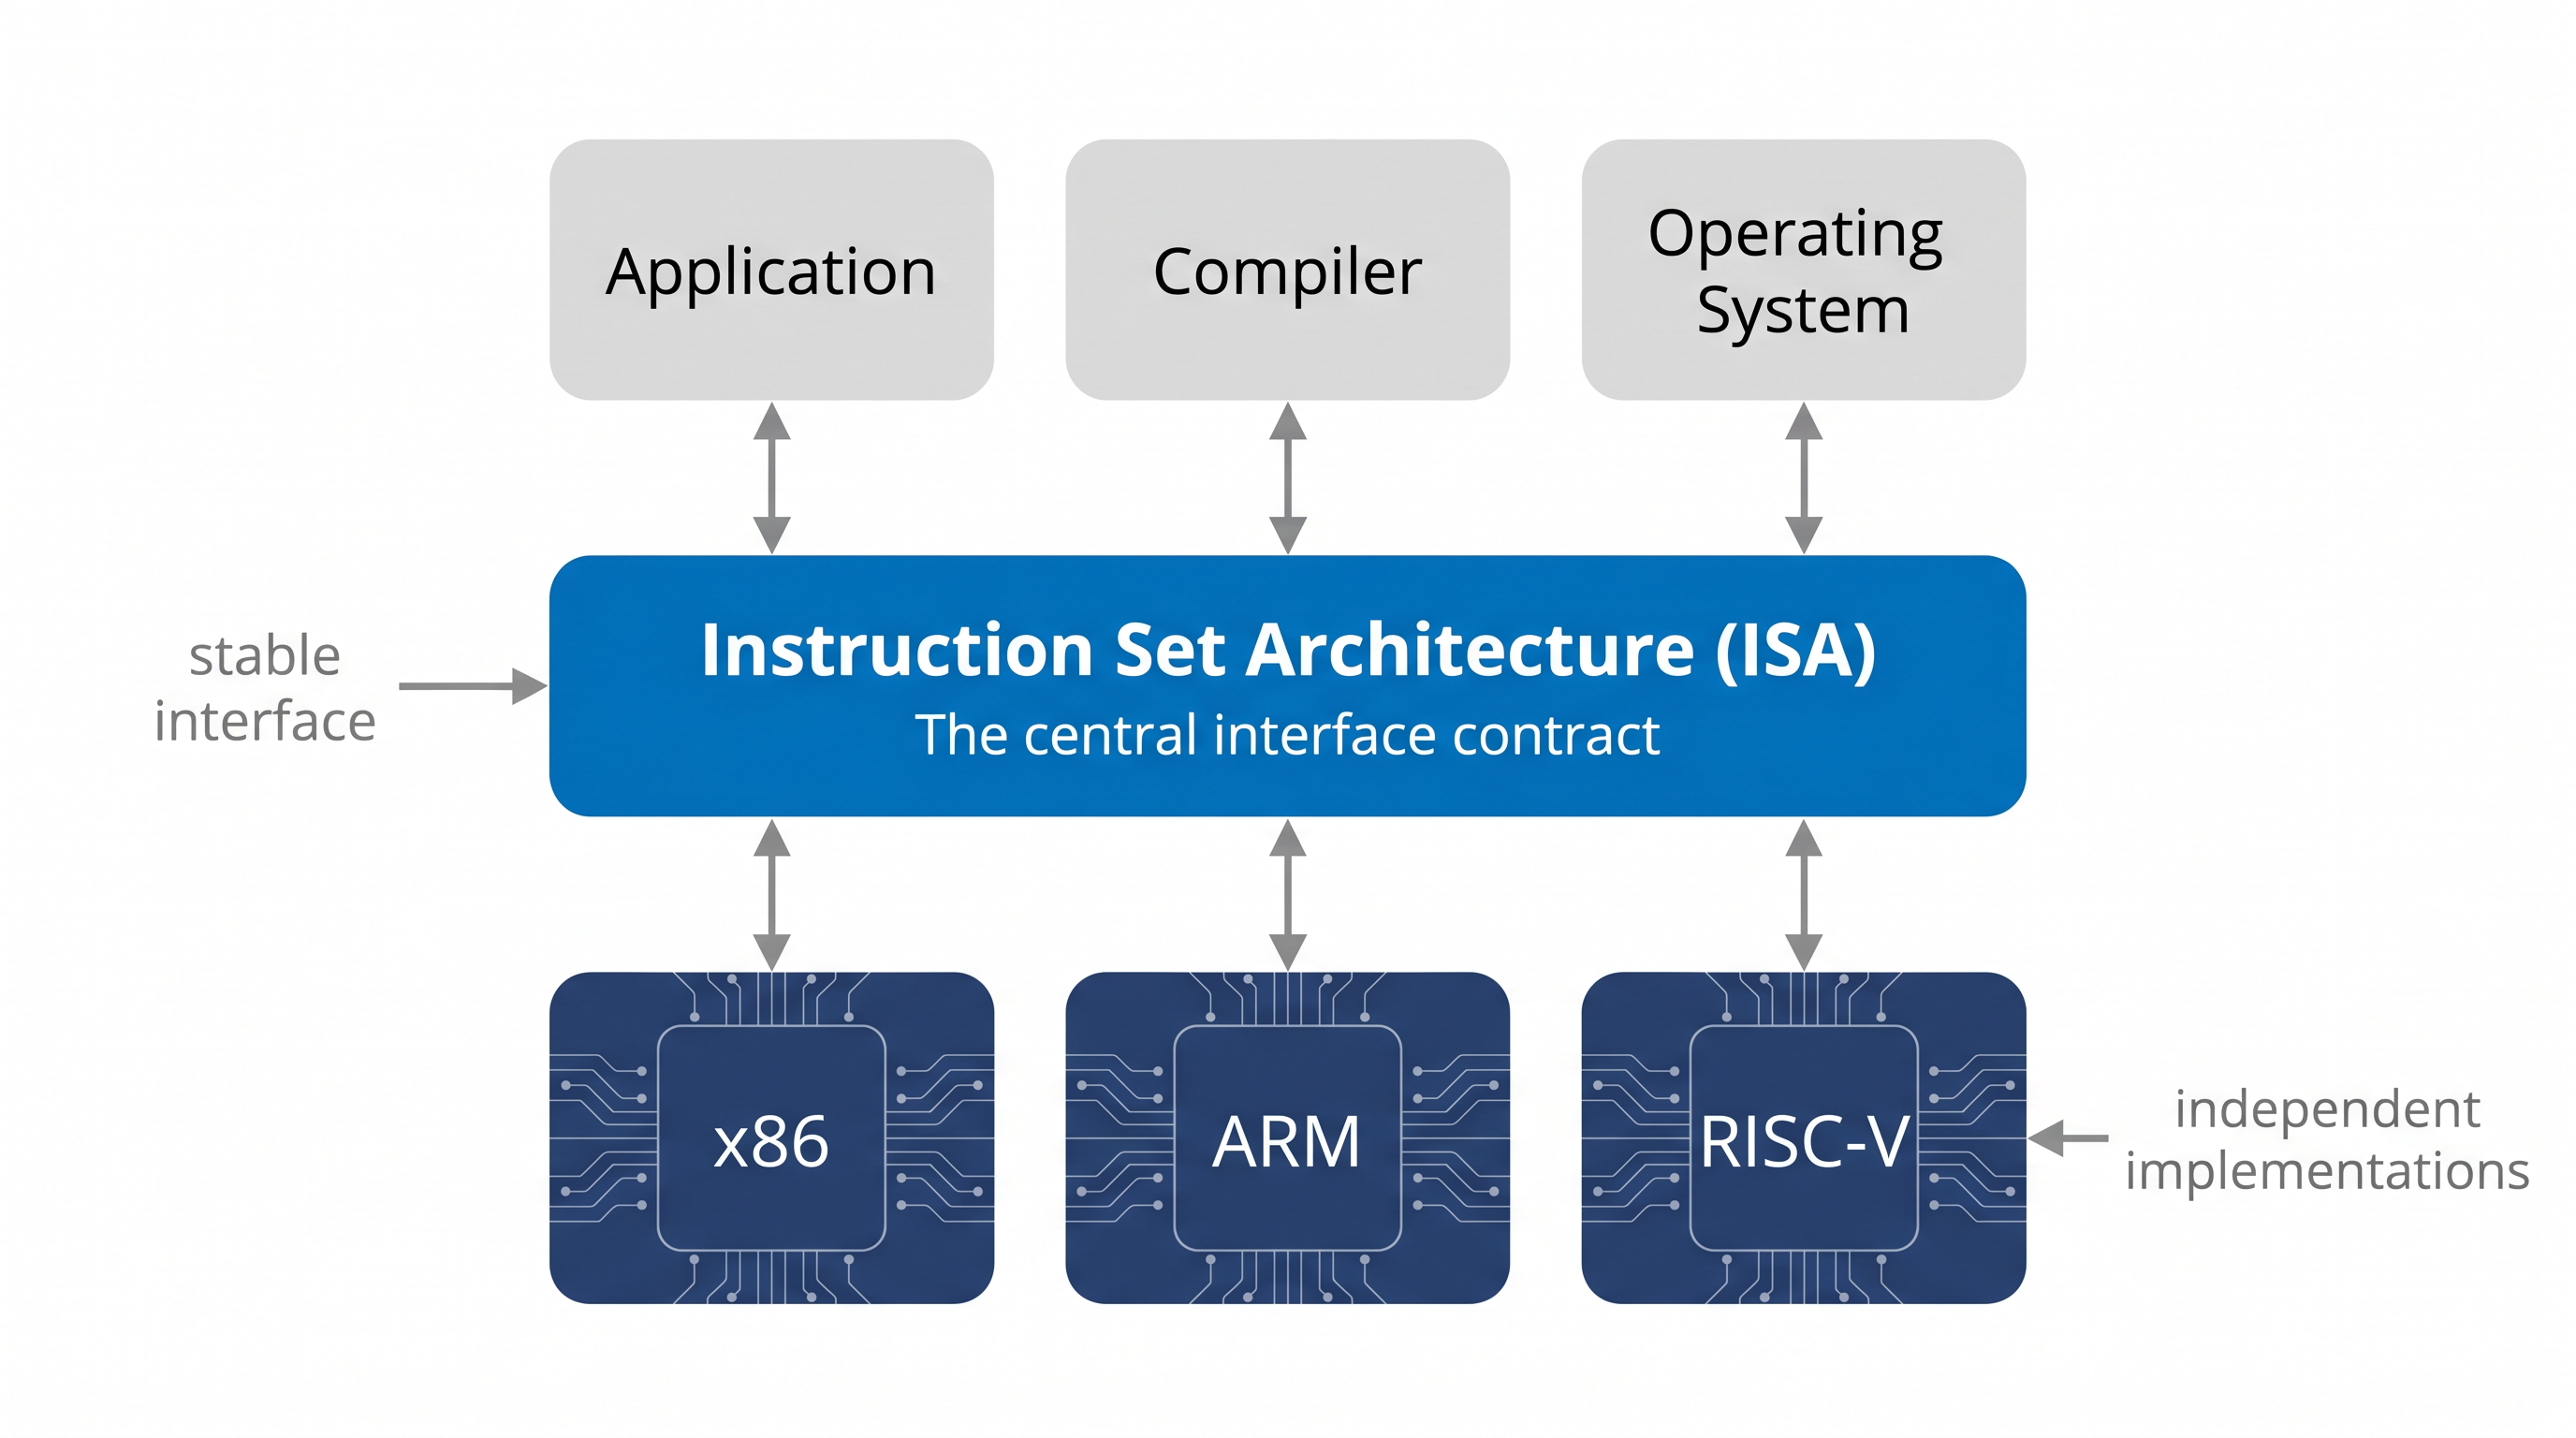
\includegraphics[width=\linewidth]{figures/generated/fig_bg_21_isa}
    \subcaption{ISA: the hardware--software contract}
    \label{fig:bg21:isa}
  \end{minipage}\hfill
  \begin{minipage}[t]{0.30\textwidth}
    \centering
    \includegraphics[width=\linewidth]{figures/generated/fig_bg_21_microarch}
    \subcaption{Microarchitecture: pipelined execution}
    \label{fig:bg21:microarch}
  \end{minipage}\hfill
  \begin{minipage}[t]{0.30\textwidth}
    \centering
    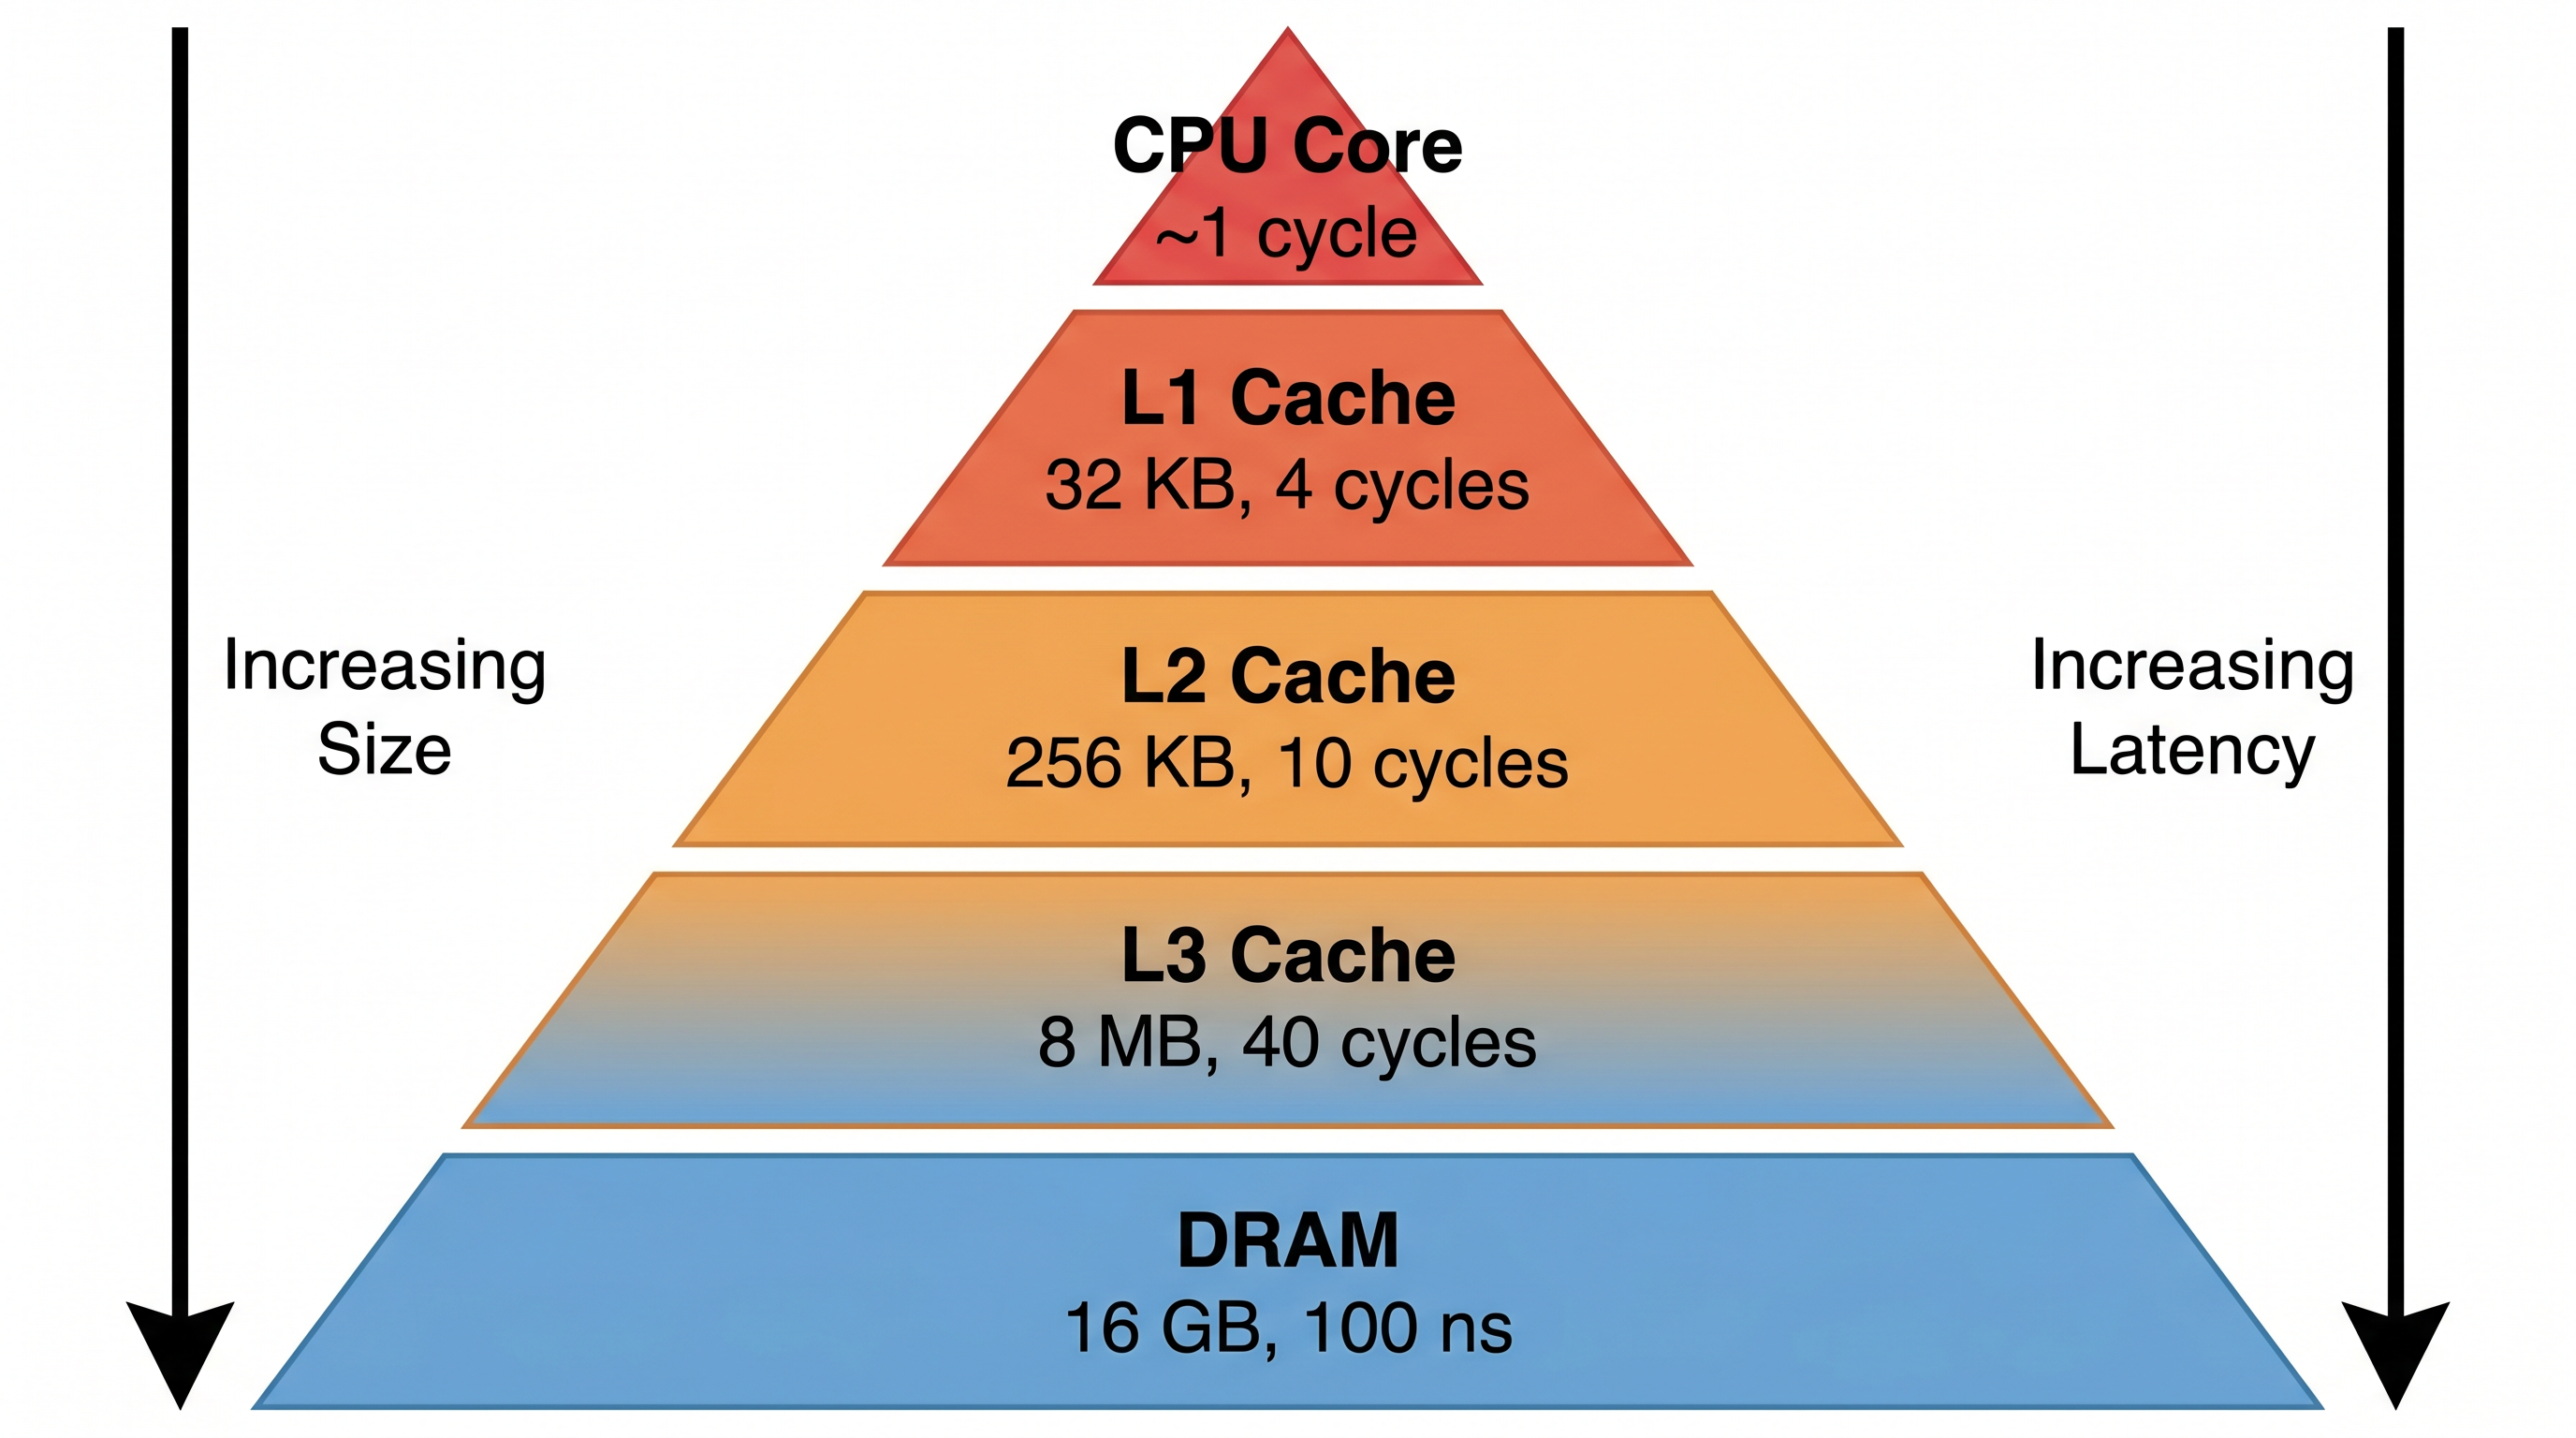
\includegraphics[width=\linewidth]{figures/generated/fig_bg_21_cache}
    \subcaption{Cache hierarchy: exploiting locality}
    \label{fig:bg21:cache}
  \end{minipage}

  \vspace{0.8em}

  \begin{minipage}[t]{0.30\textwidth}
    \centering
    \includegraphics[width=\linewidth]{figures/generated/fig_bg_21_virtualmem}
    \subcaption{Virtual memory: paging and isolation}
    \label{fig:bg21:vm}
  \end{minipage}\hfill
  \begin{minipage}[t]{0.30\textwidth}
    \centering
    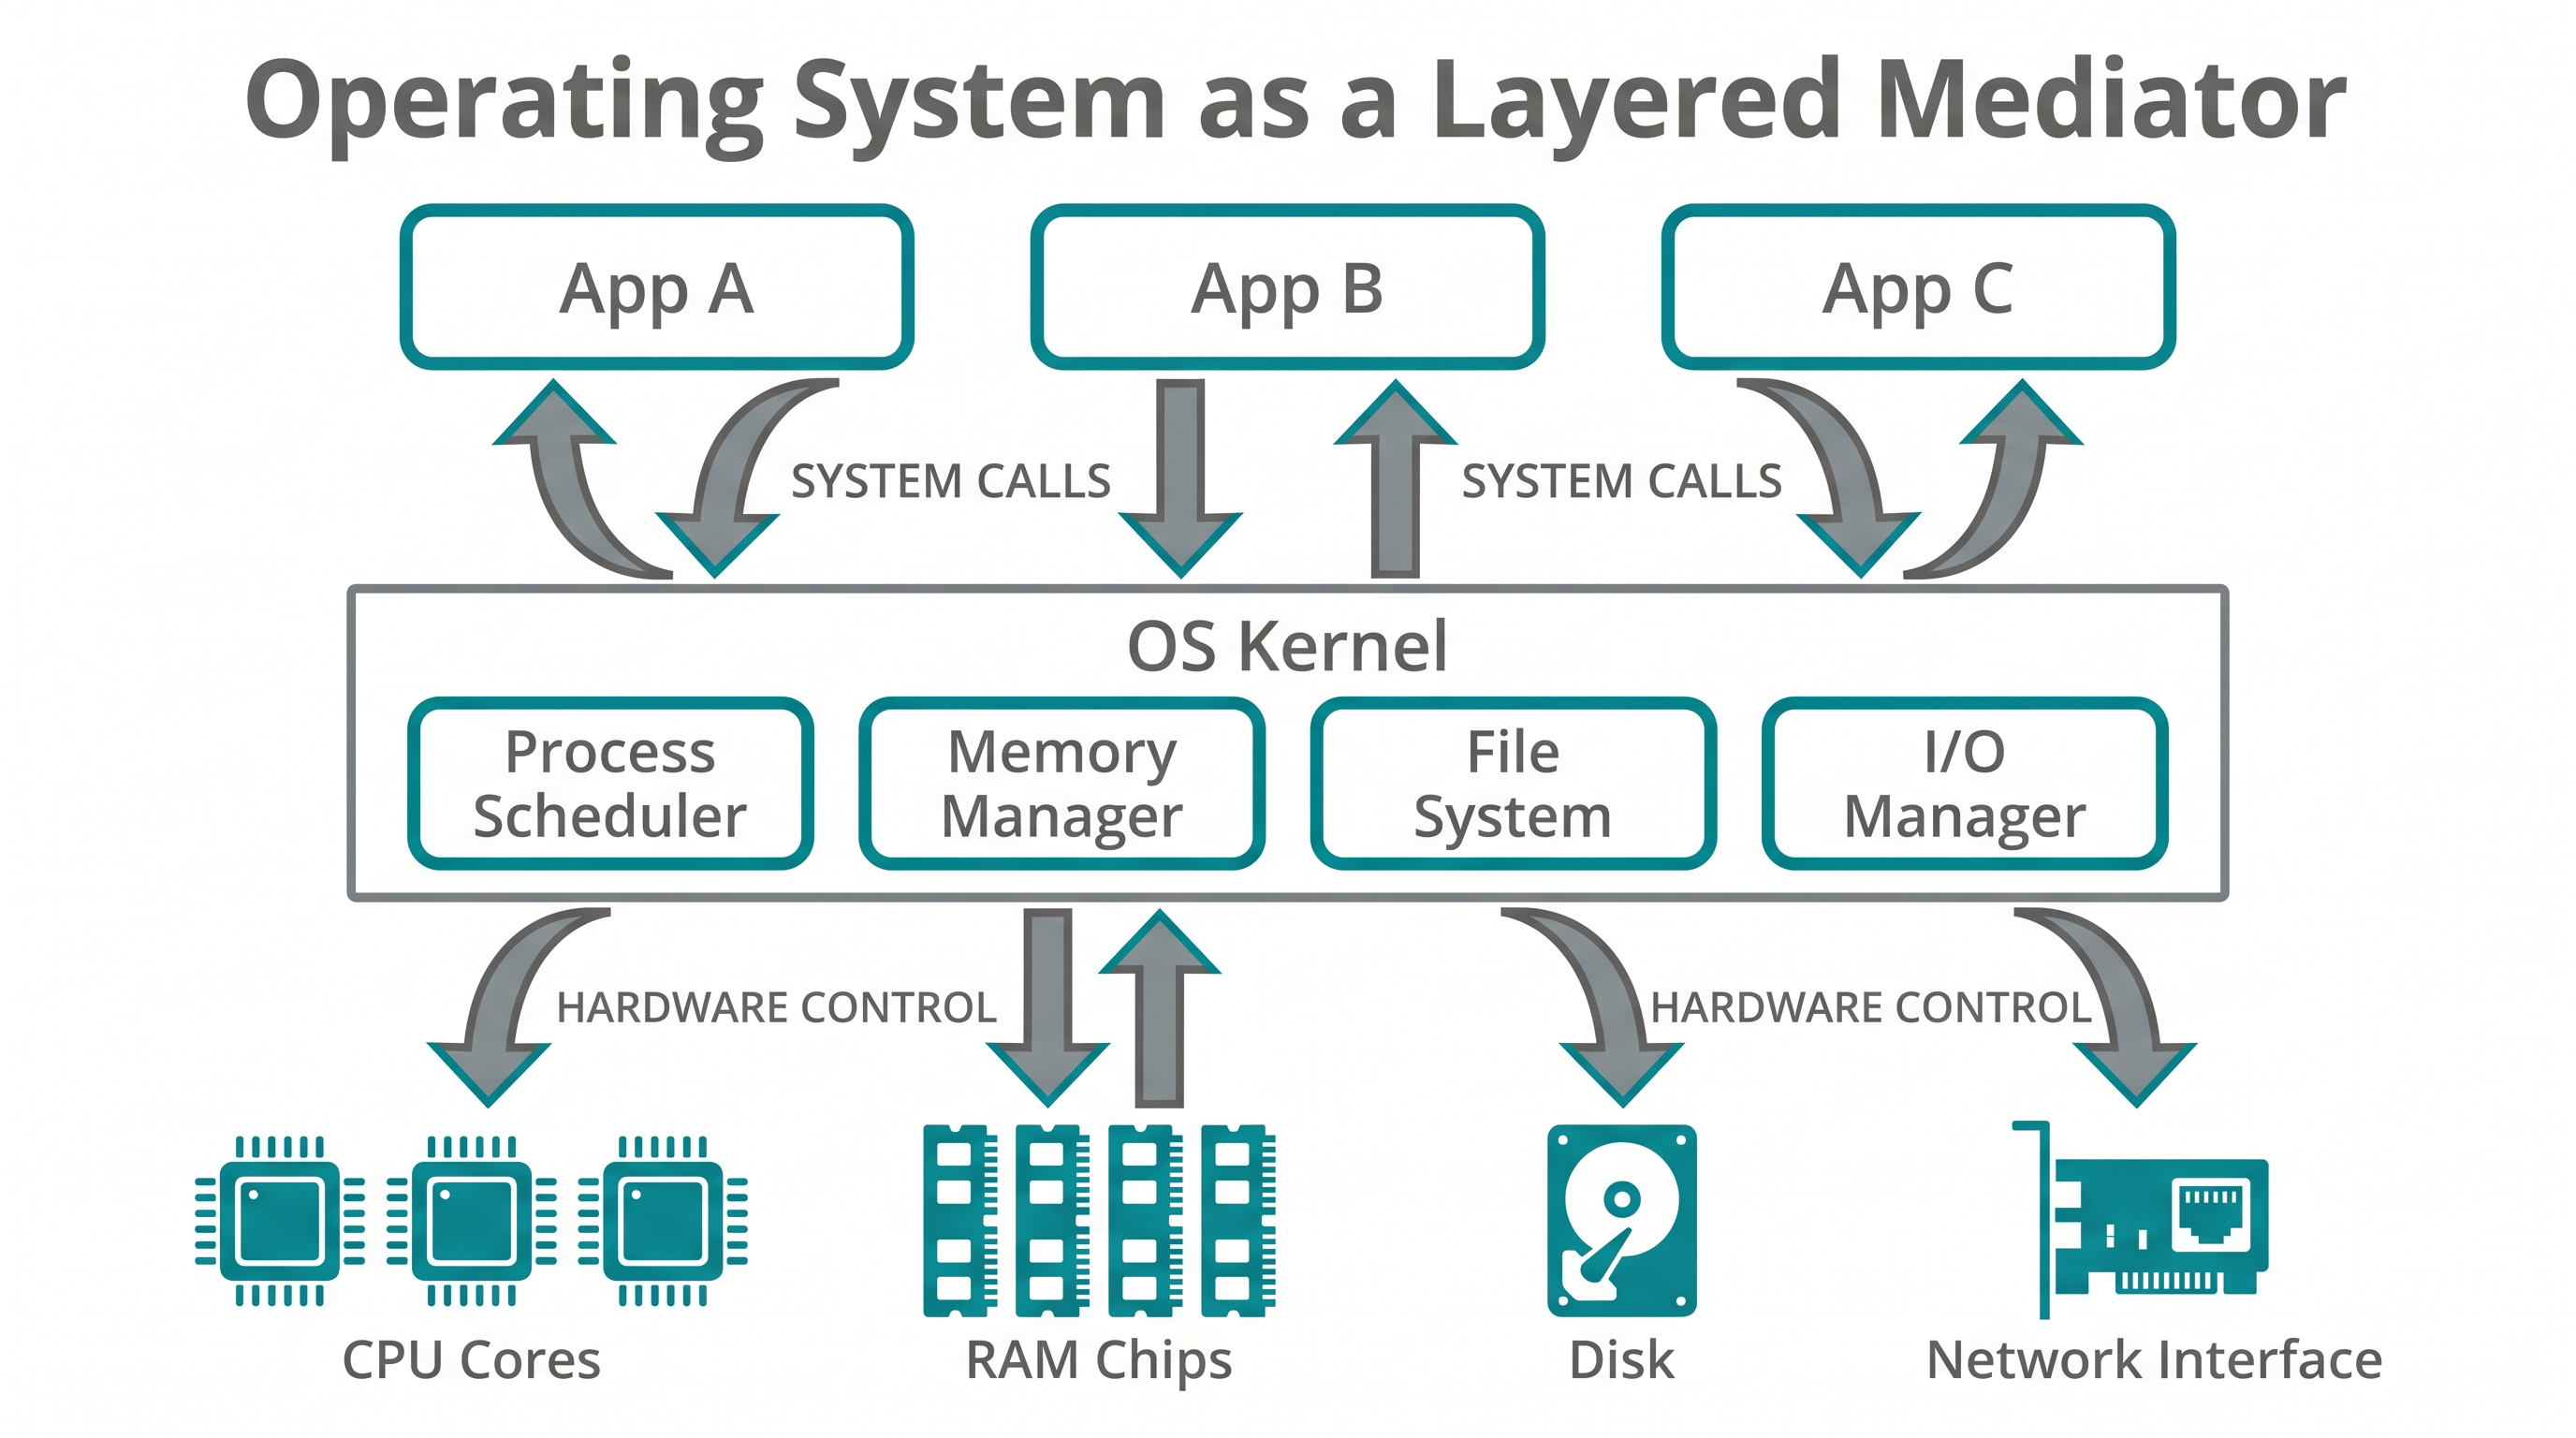
\includegraphics[width=\linewidth]{figures/generated/fig_bg_21_os}
    \subcaption{Operating system: resource management}
    \label{fig:bg21:os}
  \end{minipage}\hfill
  \begin{minipage}[t]{0.30\textwidth}
    \centering
    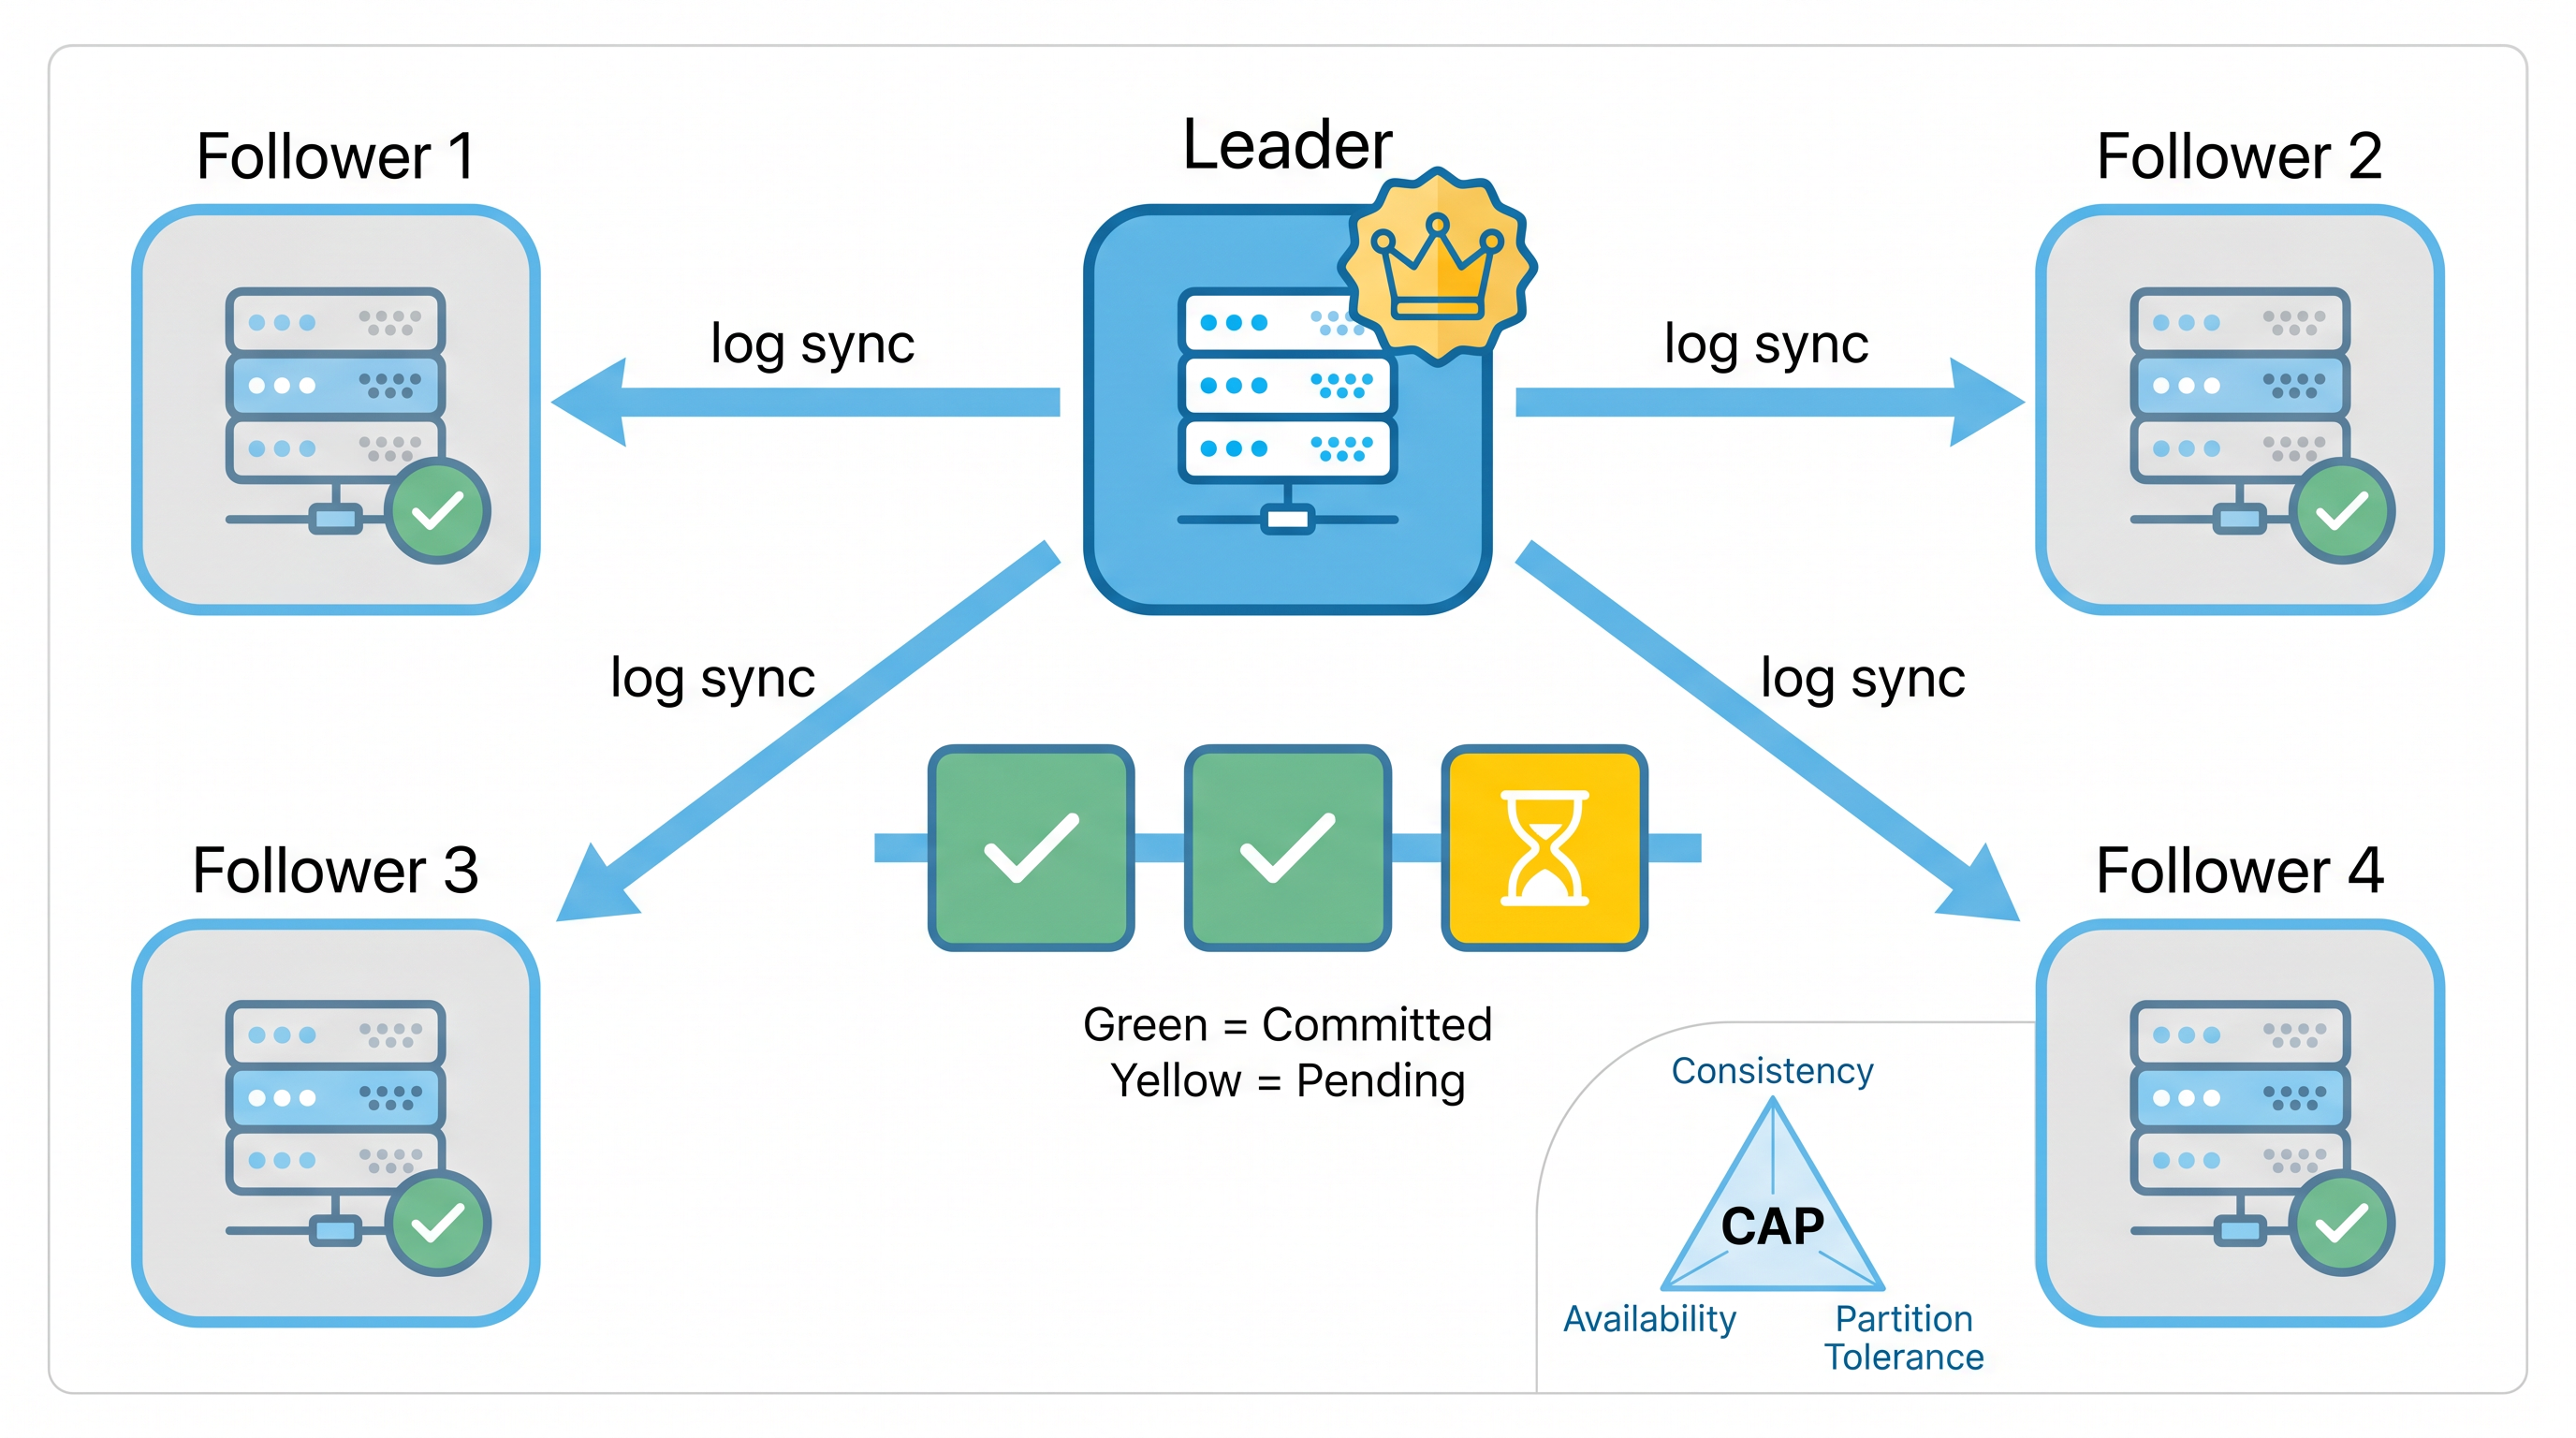
\includegraphics[width=\linewidth]{figures/generated/fig_bg_21_distributed}
    \subcaption{Distributed systems: Raft consensus}
    \label{fig:bg21:dist}
  \end{minipage}

  \caption{The six layers of the classical computing stack.
  (a)~The ISA defines a stable contract between hardware implementations and the software stack.
  (b)~Microarchitecture pipelines instruction execution across multiple stages.
  (c)~The cache hierarchy exploits temporal and spatial locality to bridge the processor--memory speed gap.
  (d)~Virtual memory maps a large virtual address space onto limited physical frames via page tables.
  (e)~The operating system mediates access to hardware resources through scheduling, memory management, and I/O abstraction.
  (f)~Distributed systems extend the stack across nodes, requiring consensus protocols to maintain correctness under failures.}
  \label{fig:bg21:classical_stack}
\end{figure}
